%%
%% ****** ljmsamp.tex 13.06.2018 ******
%%
\documentclass[
11pt,%
tightenlines,%
twoside,%
onecolumn,%
nofloats,%
nobibnotes,%
nofootinbib,%
superscriptaddress,%
noshowpacs,%
centertags]%
{revtex4}
\usepackage{ljm}
\usepackage{listings}

\lstset{
language=C++,
basewidth=0.5em,
xleftmargin=45pt,
xrightmargin=45pt,
basicstyle=\small\ttfamily,
keywordstyle=\bfseries\underbar,
numbers=left,
numberstyle=\tiny,
stepnumber=1,
numbersep=10pt,
showspaces=false,
showstringspaces=false,
showtabs=false,
frame=trBL,
tabsize=2,
captionpos=t,
breaklines=true,
breakatwhitespace=false,
escapeinside={\%*}{*)}
}

\begin{document}

\titlerunning{RANS/ILES method optimization} % for running heads
\authorrunning{L.~A.~Benderskiy, D.~A.~Lyubimov, A.~A.~Rybakov} % for running heads

\title{RANS/ILES Method Optimization\\
for Effective Calculations on Supercomuter}
% Splitting into lines is performed by the command \\
% The title is written in accordance with the rules of capitalization.

\author{\firstname{L.~A.}~\surname{Benderskiy}}
\email[E-mail: ]{leosun.ben@gmail.com}
\affiliation{Joint Supercomputer Center of the Russian Academy of Sciences - branch of Scientific Research Institute of System Analysis of the Russian Academy of Sciences, Leninsky prospect 32a, Moscow, 119334, Russia}

\author{\firstname{D.~A.}~\surname{Lyubimov}}
\email[E-mail: ]{dalyubimov@ya.ru}
\affiliation{Joint Supercomputer Center of the Russian Academy of Sciences - branch of Scientific Research Institute of System Analysis of the Russian Academy of Sciences, Leninsky prospect 32a, Moscow, 119334, Russia}

\author{\firstname{A.~A.}~\surname{Rybakov}}
\email[E-mail: ]{rybakov.aax@gmail.com}
\affiliation{Joint Supercomputer Center of the Russian Academy of Sciences - branch of Scientific Research Institute of System Analysis of the Russian Academy of Sciences, Leninsky prospect 32a, Moscow, 119334, Russia}


\firstcollaboration{(Submitted by S.~S.~Submitter)} % Add if you know submitter.
%\lastcollaboration{ }

\received{June 13, 2018} % The date of receipt to the editor, i.e. December 06, 2017

\begin{abstract}
TODO
\end{abstract}

\subclass{68N19} % Enter 2010 Mathematics Subject Classification.

\keywords{TODO.} % Include keywords separeted by comma.

\maketitle

% Text of article starts here.

\section{Introduction}

TODO

\section{Section 1}

TODO

\section{Section 2}

TODO

\section{Realization of linked border conditions}

TODO

\begin{figure}[h]
\setcaptionmargin{5mm}
\onelinecaptionsfalse
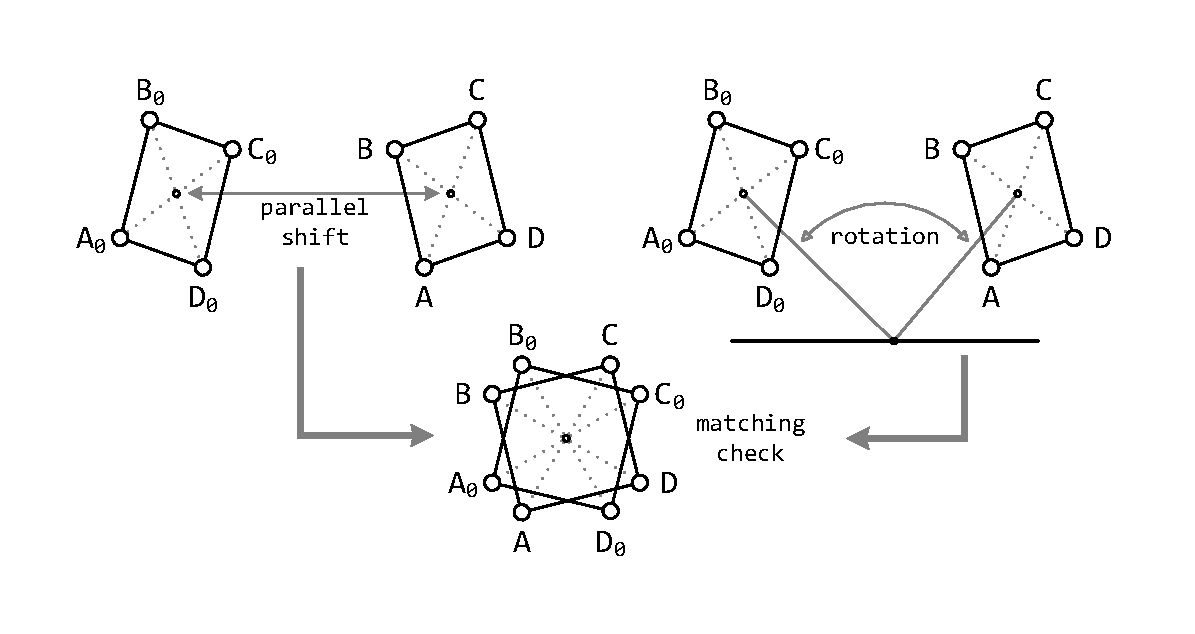
\includegraphics[width=0.95\textwidth]{pics/match3.pdf}
\captionstyle{normal}
\caption{Connection of linked border conditions to each other \\ using parallel shift and rotation around a straight line.}
\label{fig:match3}
\end{figure}

TODO

\begin{figure}[h]
\setcaptionmargin{5mm}
\onelinecaptionstrue
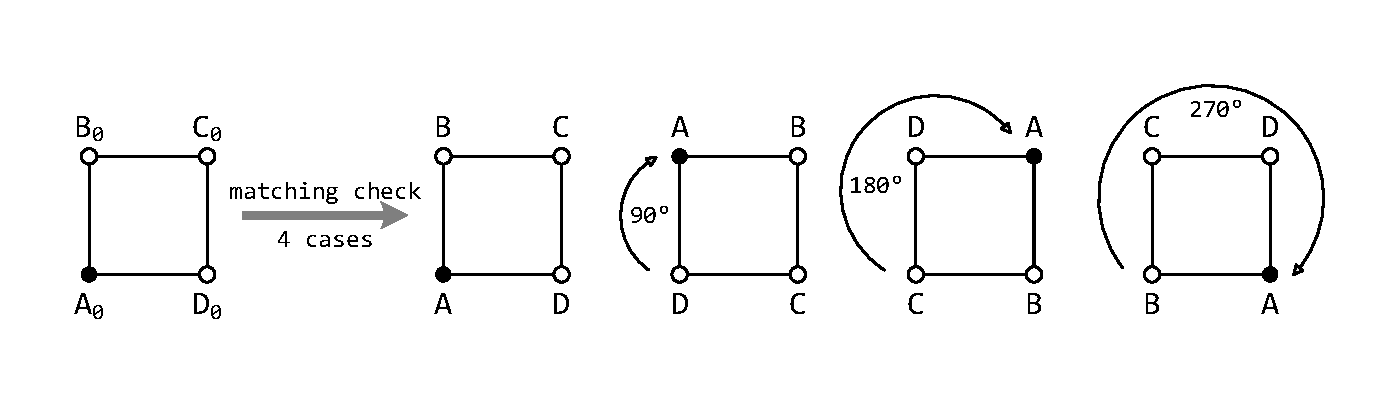
\includegraphics[width=0.95\textwidth]{pics/match.pdf}
\captionstyle{normal}\caption{Four cases for checking the coincidence of the corner points of the border conditions.}
\label{fig:match}
\end{figure}

TODO

\begin{figure}[h]
\setcaptionmargin{5mm}
\onelinecaptionstrue
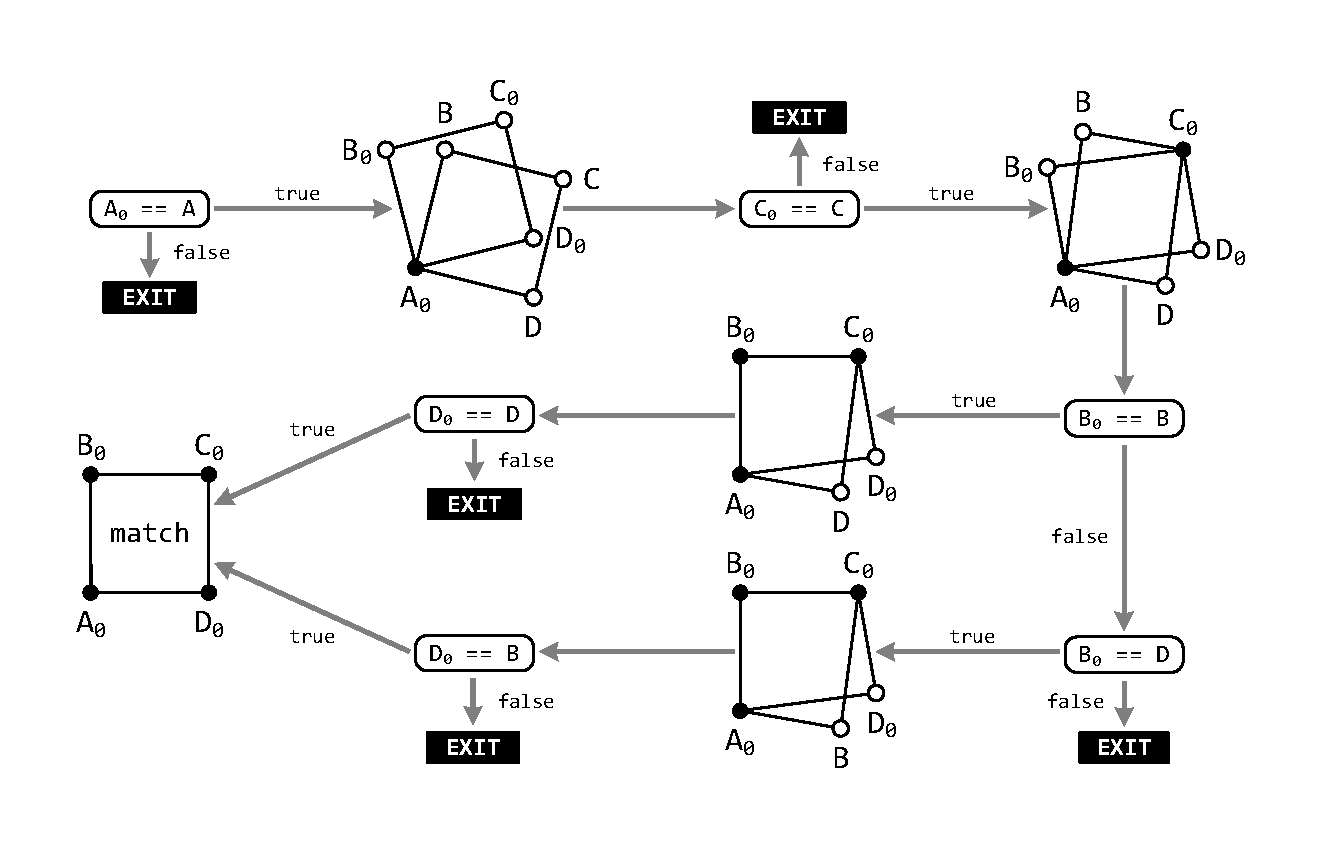
\includegraphics[width=0.95\textwidth]{pics/match2.pdf}
\captionstyle{normal}\caption{Checking the coincidence of the corner points of the border conditions.}
\label{fig:match2}
\end{figure}

TODO
        
\section{Scalability of calculations investigation \protect\\ when cutting the computational grid}

TODO

\begin{table}[!h]
\setcaptionmargin{0mm}
\onelinecaptionsfalse
\captionstyle{flushleft}
\caption{Characteristics of computational grids.}
\bigskip
\begin{tabular}{|c|c|c|c|c|}
\hline
grid description & blocks/scopes & interfaces & border conditions & linked border cond. \\
\hline
360 deg. (94.3 mln cells) & 300 & 1 796 & 1 643 & 0 \\
36 deg. (10.7 mln cells) & 30 & 152 & 204 & 14 \\
\hline
36 deg., cut for 16 proc. (10\% dev.) & 39 & 224 & 218 & 14 \\
36 deg., cut for 32 proc. (10\% dev.) & 54 & 340 & 248 & 14 \\
36 deg., cut for 64 proc. (10\% dev.) & 170 & 982 & 429 & 23 \\
\hline
36 deg., cut for 64 proc. (1\% dev.) & 383 & 2 356 & 682 & 34 \\
\hline
\end{tabular}
\label{tab:grids}
\end{table}

TODO

\begin{figure}[h]
\setcaptionmargin{5mm}
\onelinecaptionsfalse
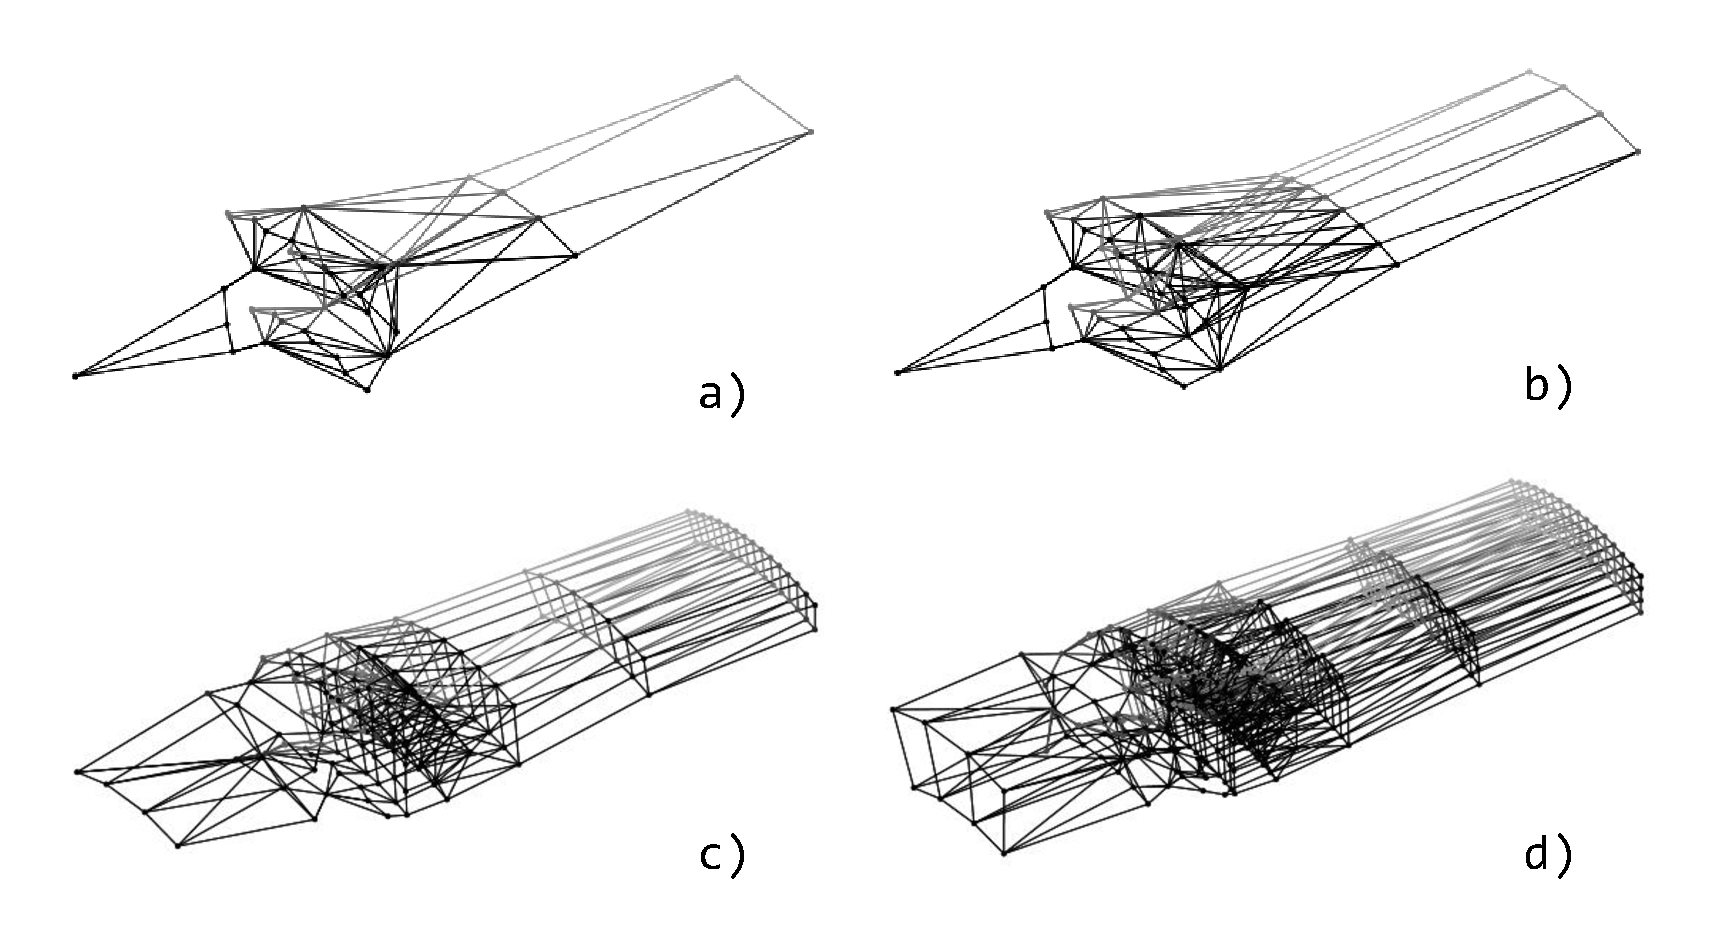
\includegraphics[width=0.95\textwidth]{pics/g_36_2.pdf}
\captionstyle{normal}\caption{Borders adjacency graphs for different cases of computational grid cutting: \\ a - cutting for 16 processes (10\% deviation), b - cutting for 32 processes (10\% deviation), \\ c - cutting for 64 processes (10\% deviaton), d - cutting for 64 processes (1\% deviation).}
\label{fig:g_36_2}
\end{figure}

TODO

\begin{figure}[h]
\setcaptionmargin{5mm}
\onelinecaptionstrue
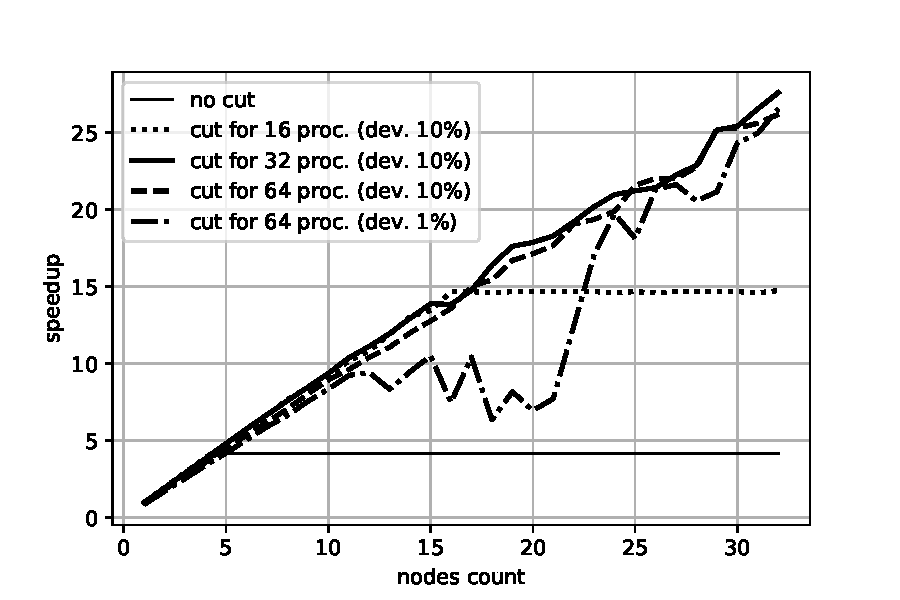
\includegraphics[width=0.95\textwidth]{pics/plot_36_scaling_2.pdf}
\captionstyle{normal}\caption{Graph scaling calculations when using different options for cutting the grid.}
\label{fig:plot_36_scaling_2}
\end{figure}

\section{Conclusion}

TODO

\begin{acknowledgments}
TODO
\end{acknowledgments}

\begin{thebibliography}{99}

% References for INTRODUCTION section.

\end{thebibliography}

\end{document}
